\section{About the dataset}
\label{sec:dataset_analysis}
% TODO: slower introduction into the section, talk about landing fields again
% TODO: elaborate why this specific dataset was used
% TODO: which hardware used for data? how collected? -> https://www.opengeodata.nrw.de/produkte/geobasis/lbi/dop/dop_jp2_f10/

The dataset which is used throughout this thesis is provided by the Ministry of the Interior of the State of North Rhine-Westphalia in Germany. With the platform GEOportal\footnote{available at \url{https://www.geoportal.nrw/}} they offer various types of maps, like topographical maps, elevation data and orthographical footage. Most of the data is available for free download in batches. The batches used in this thesis are released under the dl-de/zero-2-0 licence. This means that the data can be used for any purpose without any restrictions or conditions\footnote{see the full license text at \url{https://www.govdata.de/dl-de/zero-2-0}}.

For the purpose of this thesis there are two types of maps which prove useful. First, there is a map assembled of digital orthophotos (DOPs). A DOP is an aerial photograph of the surface of the earth. It is processed to hide effects like perspective distortions or topographic features of the landscape. Also it follows a specific map projection to denote the exact spatial extents of the photograph on the earth's surface. Because of that, DOPs are great to analyze terrain coverage and conditions. In section~\ref{sec:segmentation} DOPs are used to perform a semantic segmentation based on the terrain surface.

The second map explored in this thesis contains imagery obtained by near-infrared (NIR) spectroscopy. They are processed in the same way as the DOPs, so they are also projected onto the earth's surface with a specific map projection. NIR data is widely applied in agriculture to monitor the cultivation of herbal products like forages and vegetables. In this thesis the NIR imagery is used to approximate vegetation density for specific regions (see section~\ref{sec:vegetation_analysis}).

\subsection{Getting the dataset}
Both the DOP and NIR datasets are provided by the Ministry of the Interior in a few different ways. To get a quick overview, there is an online viewer for most of the map types available at \url{https://www.tim-online.nrw.de/tim-online2/}. For some specific maps like the DOPs they host a Web Map Tile Service, which allows to access the data with geographic information systems (GIS) like QGIS\footnote{QGIS is a free and open-source GIS application available at \url{https://qgis.org/}}. Since these options require a continuous network connection, it is preferred to get a local copy of the dataset and work with that.

For that purpose, the GEOportal has a separate download section. There you can choose the regions and map types you need and download them in a compressed bundle. The bundle contains map tiles in the JPEG 2000 file format. This is an image format that has a dense compression rate and directly contains the georeferencing information for each tile. To have a wide range of terrain types with broad variety included, we use the data for the Municipality of Arnsberg and its surroundings. This concludes to a download size of $11.5~\text{Gigabytes}$ with around $248.49~\text{km}^2$ of terrain, where each pixel represents a $10\times 10~\text{cm}$ square in scale.
% TODO: JPEG 2000 not very widely accepted

It is possible to download both DOP and NIR data together in a single bundle. The JPEG files then contain four bands of pixel information. The first three bands make up the red, green and blue colors for the DOPs. And the last band provides the scalar output of the NIR spectroscopy scan.

% TODO: show some example images from the dataset, maybe later?
% TODO: demonstrate the limits of practical feasibility, maybe later?

\subsection{Preparing the dataset}
Before the data is ready to be used for training the models, some preprocessing steps have to be performed. In figure~\ref{fig:data_preprocessing} the whole preparation process is summarized briefly. The present and following sections focus on importing the whole data into a standardized database. Afterwards, Section~\ref{sec:image_export} explains the steps to prepare the data for the use of training. Most processing steps are automated with Python scripts, which can be found in~\cite{thesis-code}.

\begin{figure}[h]
    \centering
    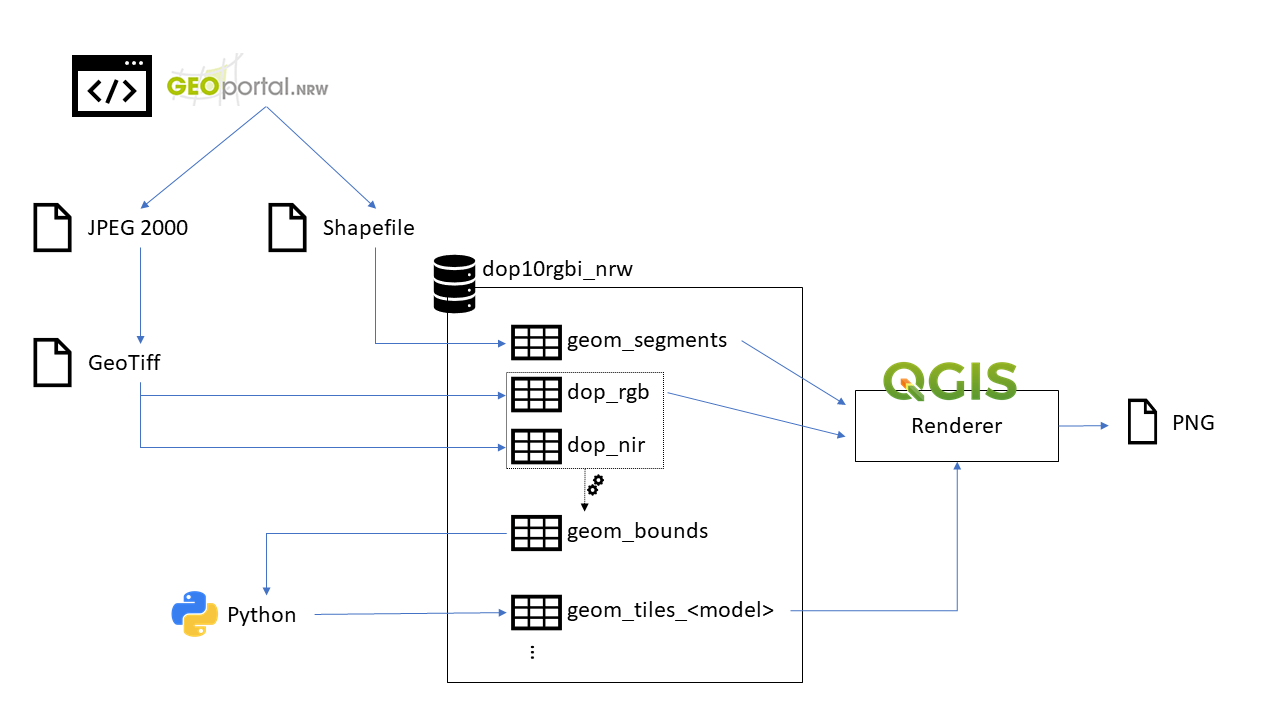
\includegraphics[width=0.9\textwidth]{images/data_preprocessing}
    \caption{Summary of the Data Preprocessing Steps}
    \label{fig:data_preprocessing}
\end{figure}

As a first step, the whole dataset is imported into a spatial database system. By doing that, it is very easy to export the data in various data formats and tile sizes required by the reference architectures (see section~\ref{sec:ref_archs}). PostgreSQL\footnote{see \url{https://www.postgresql.org/}} is a powerful open-source database system. Together with PostGIS\footnote{see \url{https://postgis.net/}}, a free and open-source extension for PostgreSQL, it is capable of performing spatial operations on image rasters and vector objects. For example, it adds database functions to merge raster tiles, calculate intersection regions or determine bounding boxes.

The PostGIS installation contains a few shell tools to import data into the database. Unfortunately, they do not support the JPEG 2000 image file format. Before the import of the data can take place, it has to be translated to one of the supported formats first. One of the most widely used formats is GeoTiff. The Tiff file standard is great, because it consists of a baseline section which contains the image information, and a meta section which can contain all kinds of meta information. For example, it can be used to store georeferencing information, which PostGIS is able to use for importing GeoTiff files.

To convert the files from JPEG 2000 to GeoTiff, we use the \emph{Geospatial Data Abstraction Library} (GDAL). This is a tool collection which acts as an abstraction layer for various geospatial data formats. It also includes a shell tool to translate several georeferenced image file formats, including JPEG 2000 and GeoTiff. The file \texttt{scripts/jp2\_to\_tif.sh} in~\cite{thesis-code} shows a bash script using the \texttt{gdal\_translate} tool to convert all the JPEG 2000 files to the GeoTiff format.

With the files in GeoTiff format it is now possible to use the \texttt{raster2pgsql} tool to import them into a PostGIS raster table. The whole import process is automated with a Python script (see file \texttt{scripts/tif\_to\_raster.py} in~\cite{thesis-code}). It assumes that there is a database called \texttt{dop10rgbi\_nrw} with the PostGIS extension enabled.

In the first step, the script creates two database tables named \texttt{dop\_rgb} and \texttt{dop\_nir}. The \texttt{dop\_rgb} table has a PostGIS raster column with three raster bands to hold the color information for the DOPs. Simultaneously, the \texttt{dop\_nir} table also has a PostGIS raster column with only one raster band for the NIR values. It is reasonable to separate the color and NIR values as they will be used for different tasks later on.

After the tables are created, the script loops through all the GeoTiff files and calls the \texttt{raster2pgsql} tool for every single one. That call returns some SQL insert statements enriched with the raster information in a binary representation. To execute those statements, it is possible to simply pipe the output of \texttt{raster2pgsql} into a \texttt{psql} command which is connected to the database.

The \texttt{raster2pgsql} tool provides a lot of arguments to properly configure the import of the data. Obviously it needs to know the name of the file to import and the name of the database table to insert the data to. For performance reasons it is very important to set an appropriate tile size for the raster. The original tile size of the GeoTiff files ($10000\times 10000$ pixels) was assessed to be too large. After some experiments, a tile size of $1000\times 1000$ pixels was found to work best for both the initial import and the later processing of the raster.

Another major configuration is the spatial reference id (SRID). It also has to be passed as an argument, to ensure the data is imported correctly. The SRID indicates the map projection that is used to map the raster to the earth's surface. The dataset is provided with the SRID 25832. This SRID does not cover the entire globe, but only a rectangular area on the European continent. Therefore it offers a high precision (without too much distortion) in that area and is widely used for maps in Central Europe.

After all GeoTiff files are imported, the Python script creates a Generalized Search Tree (GiST) index for both tables. This takes into account the spatial character of the data and thus speeds up spatial queries (like merging, intersecting) on the tables significantly. For the same reason, the Python script also enforces some constraints on the raster columns of the tables. This makes sure that all the raster tiles share common properties like tile size, SRID or the number of raster bands.

As a last step of the Python script, it creates one last table named \texttt{geom\_bounds}. This table holds a single PostGIS geometry object defining the exact boundaries of the raster tiles. That allows for a quick way to calculate if a given region is included in the spatial extents of the raster without having to process the whole raster table all the time.

Figure~\ref{fig:dop_rgb_all} shows the color bands of the whole dataset and its location in Germany. To show the granularity of the data, one region is enlarged and shown in full resolution. One pixel in the dataset represents $10\times 10$ decimeters in real-world scale. As can be seen in figure~\ref{fig:dop_rgb_all}, it is easily possible to detect objects like trees, cars or buildings with such a high resolution. Therefore, the data provides sufficient information for the segmentation of land usage.

% TODO: adjust figure, show map of Germany, zoom to whole dataset, then zoom to high-resolution tile
\begin{figure}[h]
    \centering
    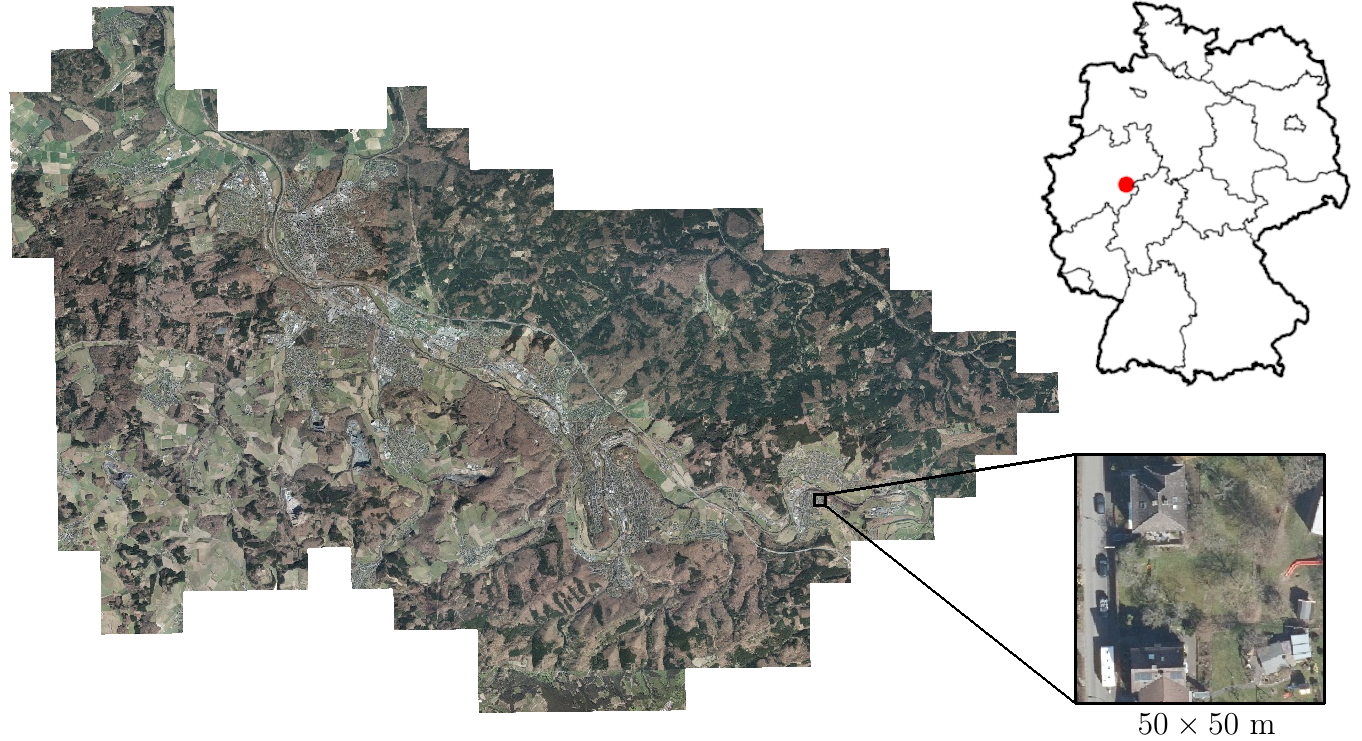
\includegraphics[width=\textwidth]{images/dop_rgb_all}
    \caption{The DOPs in the dataset}
    \label{fig:dop_rgb_all}
\end{figure}

\subsection{Preparing the labels}
As explained in section~\ref{sec:dl_paradigms}, for supervised training you need to provide the model with a pair of input and expected output. The DOPs explained in the previous section function as input for the model. To train the model for segmentation, another prerequisite is to have some segmentation examples prepared. Usually this task is done manually by lining out the segments of a tile and then assigning a category to each segment.

To reduce the amount of work, we use another dataset from the GEOportal called Digital Basic Landscape Model~\cite{base-dlm20}. It describes topological features of the landscape in a vector data format. Besides other things like \WIP{points of interest}, it includes regions categorized by their respective land use. The dataset is available for free download and also permits any use within the dl-de/zero-2-0 license. With some transformation the data fits perfectly for the use as labels during the training of a model.

The categorized regions are provided as Shapefiles. Shapefile is a specific data format for vector-based geospatial objects. To have all data in a single source system, the Shapefiles are imported into the PostGIS database. This also makes it easier to export the segmentation information later on for different tile sizes. Again, the import process is automated with a Python script (see file \texttt{scripts/shp\_to\_geom.py} in~\cite{thesis-code}).

PostGIS includes a tool called \texttt{shp2pgsql} to import Shapefiles into a database table with a PostGIS geometry column. It takes into account all the metadata that is listed in the Shapefile and creates separate columns for those values. The Python script loops over all the required Shapesfiles and calls the \texttt{shp2pgsql} tool passing some arguments like the target SRID. At first, each file is imported in its own database table. This is because each file contains a specific set of meta information resulting in different table layout for each file. The categorized regions are now represented as PostGIS geometry objects.

The original Shapesfiles enclose all regions of the State of North Rhine-Westphalia. Since the DOP und NIR datasets only consist of a smaller subregion, all geometry objects are cropped to that subregion in the next step. Geometry objects that are located outside of the boundaries are dropped entirely. During this process, the tables of the different Shapefiles are merged into one single table. This resulting table has columns for an internal id, the object type, a textual object description and for the geometry object itself. As all the other meta information contained in the Shapefiles is not needed, it is dropped in this step.

The Shapefiles contain a few more categories than the segmentation in this thesis aims for. For example, the difference between industrial zones and housing zones is negligible for the purpose of emergency landings. Thus, the categories are mapped to six predefined supercategories:
\begin{itemize}
  \setlength\itemsep{1mm}
  \item water
  \item buildings
  \item agriculture
  \item forest
  \item urban greens
  \item traffic
\end{itemize}
The mapping between the categories of the Shapefiles and the chosen supercategories is to be found in table~\ref{tab:category_mapping}.

\begin{table}[]
\centering
\small
\caption{Mapping from Shapefile objects to segmentation categories}
\label{tab:category_mapping}
\begin{tabular}{|l|l|l|l|}
\hline
\textbf{Shapefile} & \textbf{Object Code} & \textbf{Object Description}    & \textbf{Segmentation Category} \\ \hline
gew01\_f           & 44001                & running water                  & water                          \\ \hline
gew01\_f           & 44005                & harbor dock                    & water                          \\ \hline
gew01\_f           & 44006                & stagnant water                 & water                          \\ \hline
sie02\_f           & 41007                & specialized regions            & buildings                      \\ \hline
sie02\_f           & 41009                & cemetery                       & urban greens                   \\ \hline
sie02\_f           & 41002                & industrial zone                & buildings                      \\ \hline
sie02\_f           & 41010                & housing zone                   & buildings                      \\ \hline
sie02\_f           & 41008                & sports, recreation          & urban greens                   \\ \hline
sie02\_f           & 41005                & quarry, surface mining         & buildings                      \\ \hline
veg01\_f           & 43001                & agriculture                    & agriculture                    \\ \hline
veg02\_f           & 43002                & forest                         & forest                         \\ \hline
veg03\_f           & 43003                & woody, undergrowth             & forest                         \\ \hline
veg03\_f           & 43004                & heath                          & forest                         \\ \hline
veg03\_f           & 43007                & uncultivated zones             & agriculture                    \\ \hline
ver01\_f           & 42009                & urban squares                  & traffic                        \\ \hline
ver01\_f           & 42001                & road traffic                   & traffic                        \\ \hline
ver03\_f           & 42010                & rail traffic                   & traffic                        \\ \hline
\end{tabular}
\end{table}

The last step is to merge all geometry objects of the same category. I. e. the final table only contains six geometry objects, one for each category. This was done for convenience and performance reasons, since almost all operations performed on this table include some way of merging the geometry objects of the same category.

Figure~\ref{fig:dop_label_all} depicts the segmentation for the whole dataset with a color encoding. The most dominant categories are clearly forest and buildings. Water and traffic zones only take up a very small area and both are barely visible because of the scale of the illustration. The imbalance of the categories is an issue which is further addressed in section~\ref{sec:dataset_considerations}

% TODO: show mapping from categories to colors
\begin{figure}[h]
    \centering
    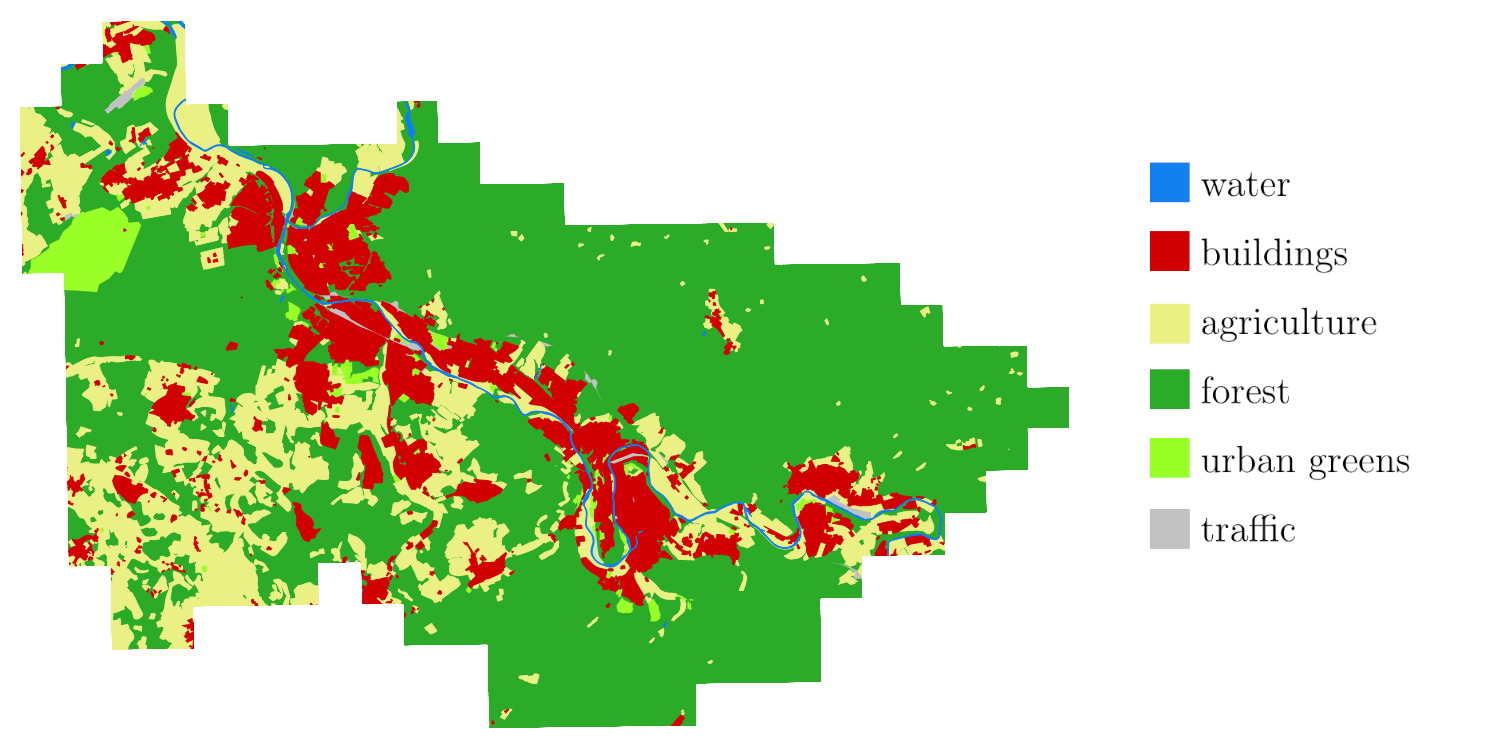
\includegraphics[width=\textwidth]{images/dop_label_all}
    \caption{The labels in the dataset}
    \label{fig:dop_label_all}
\end{figure}

\subsection{Export images for training}
\label{sec:image_export}
% TODO: confirm numbers for training/querying time
At this stage, all the data required for the training of network models is contained in the PostgreSQL database and can be queried in regions of arbitrary tile size. While it is possible to query each tile live during training, this is highly inefficient. Since the same data is fed into the network multiple times, the same query result would have to be computed multiple times during a training run (i.~e. once per epoch). Also, doing a full round of backpropagation with a single tile is by far faster than executing a query for a single tile. Depending on the architecture of the network and the available hardware, a single pass of backpropagation usually takes around \WIP{$500~\text{ms}$} at most. Compared to that, the database query for a single tile measures on average to \WIP{$x~\text{ms}$}.

One common way to use more of the available processing power for the actual training, all tiles are precomputed and saved in well-sized batches on a hard drive. That way, they only need to be loaded into memory and can then be used directly. However, depending on batch size and the hard drive's reading speed this might leave the hard drive as bottleneck. In the end, the process of feeding the data into the network is a balancing act between factors such as data compression, preprocessing pipelines and hardware availability.

% TODO: reference the correct section
For this thesis, the data is exported from the database and saved as image files in PNG format. This format offers a good tradeoff between file size on the hard drive and processing time required to decode the data. The width and height of the images depends on the shape of the input layer of the network to train and will thus be discussed later on in \WIP{section~\ref{sec:segmentation}}. Each tile is stored in a separate file. That way it is very easy to randomize the order of the images for each epoch of the training, which helps in learning generalized weights.

The PNG image format is used for both the DOP footage and the segmentation labels. For the DOPs this works great, because they contain three color bands that can be stored in the RGB channels of a PNG file. It was found to be better for training if the input values are normalized to range $[0, 1]$ before feeding them to a network \WIP{SOURCE}. Since the PNG files use 8 bit per color, this normalization can be achieved by dividing the color values by $255$.

In the image files the labels use color-encoding to differentiate between the categories. However, this is a bad representation for training, since the distance of the colors in the color space does not correlate with the similarity of the terrain types. This means the colors chosen for the categories would influence the segmentation predictions made by the network. Thus, after reading a label from a PNG file it is transformed to one-hot encoding. In one-hot encoding, each pixel is assigned a vector with one value per category. The value for the category is set to $1$ if the pixel belongs to that specific category, and $0$ otherwise. That way, the distance between the categories is equal for each pair of categories, i.~e. there is no correlation between categories. The translation from color-encoding to one-hot encoding is done by simply mapping the color vectors to their respective one-hot encoded representation.

While the exact tile and label size depends on the network architecture, there is a general process how the image tiles are extracted from the database. This process is automated with multiple Python scripts (see \texttt{scripts} folder in~\cite{thesis-code}) . The first step is to define the bounding boxes of all tiles for a specific network architecture in a separate table within the database. Each bounding box is represented by a rectangular PostGIS geometry object. It is important to line up the tiles precisely with the DOP raster, so that the raster pixels are not distorted or cut off during the export. This does not matter for the labels, because they are stored in a vector format which is not based on pixels.

To extract the image files for those tile definitions, one straightforward way would be to join the raster table \texttt{dop\_rgb} with tile table containing the tile geometries using the PostGIS \texttt{ST\_Union} and \texttt{ST\_Intersection} functions. However, this was found to take a very long time to compute. Instead, a geospatial visualization software called \emph{QGIS} was used to do those computations. It offers a Python API which allows to run batch exports of a PostGIS raster table according to the bounding boxes defining the tiles.

The Python script to export all image files with QGIS can be found in the \texttt{scripts} folder in~\cite{thesis-code}. Before running the script, QGIS has to be configured with all the layers necessary to render the tiles. QGIS offers to connect directly to a PostgreSQL database with the PostGIS extension. The raster columns from the database tables \texttt{dop\_rgb} and \texttt{dop\_nir} can simply be loaded as raster layers. For the segmentation labels multiple layers are required, each representing one category with a specified color. Thus, the geometry column from the \texttt{geom\_segments} table is loaded multiple times, each time filtered by a different segmentation category.

After all the layers have been configured, the script for the export can be executed. It reads all the tiling information from the database and distributes the rendering tasks to a few QGIS worker threads. Each worker thread is responsible for rendering the specific part of the map layers and saving it as PNG image file.

Since the tiles have been precisely aligned with the raster data, the RGB and NIR image files are pixel-perfect copies of the original dataset. However, as the labels are converted from vector space to pixel space during the export, QGIS performs color interpolation on the boundaries between adjacent segments. This is disadvantageous, because the interpolated pixels are no longer clearly assigned to a single category. To overcome this issue, another Python script iterates over all the label files and assigns proper colors to the interpolated pixels according to adjacent pixels.

Because of that process, it can happen that the segmentation maps in the exported label files slightly deviate from the labels provided in the initial dataset. However, in any case the difference is less than a few decimetres, which is acceptable in the context of this thesis.

After the export process is done, the images are ready to use for training. Figure~\ref{fig:dop_with_labels} shows some examples of images with their respective labels.

\begin{figure}
    \newcommand{\DopLabelImageWidth}{0.23\textwidth}
    \centering
    \hfill
    \begin{subfigure}{\DopLabelImageWidth}
        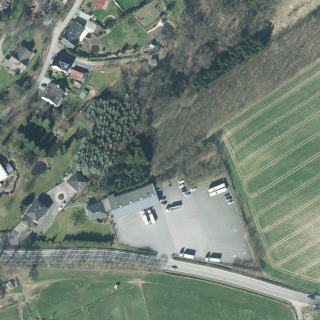
\includegraphics[width=\textwidth]{images/186_image}
    \end{subfigure}
    \hfill
    \begin{subfigure}{\DopLabelImageWidth}
        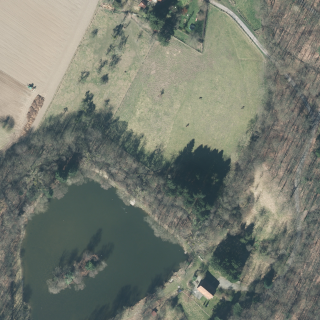
\includegraphics[width=\textwidth]{images/583_image}
    \end{subfigure}
    \hfill
    \begin{subfigure}{\DopLabelImageWidth}
        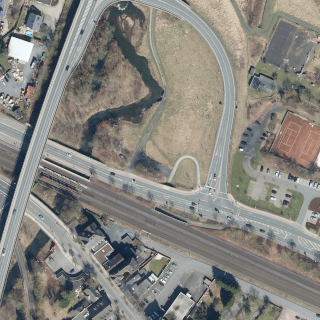
\includegraphics[width=\textwidth]{images/2281_image}
    \end{subfigure}
    \hfill
    \begin{subfigure}{\DopLabelImageWidth}
        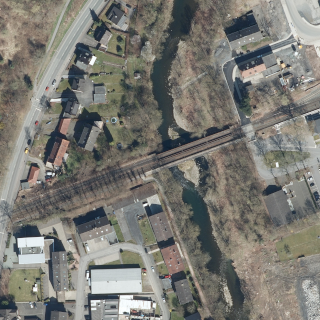
\includegraphics[width=\textwidth]{images/3589_image}
    \end{subfigure}
    \hfill

    \vspace{3mm}

    \hfill
    \begin{subfigure}{\DopLabelImageWidth}
        
\includegraphics[width=\textwidth]{images/186_label}
    \end{subfigure}
    \hfill
    \begin{subfigure}{\DopLabelImageWidth}
        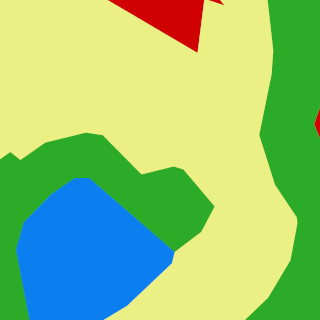
\includegraphics[width=\textwidth]{images/583_label}
    \end{subfigure}
    \hfill
    \begin{subfigure}{\DopLabelImageWidth}
        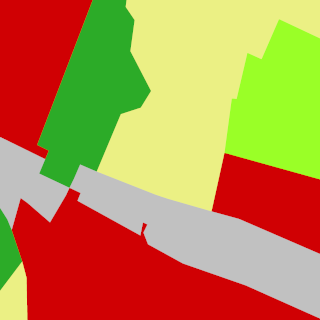
\includegraphics[width=\textwidth]{images/2281_label}
    \end{subfigure}
    \hfill
    \begin{subfigure}{\DopLabelImageWidth}
        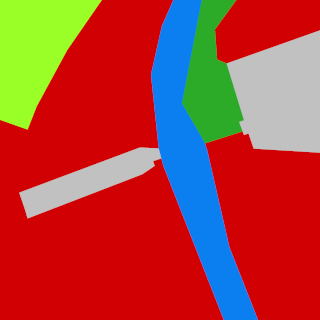
\includegraphics[width=\textwidth]{images/3589_label}
    \end{subfigure}
    \hfill

    \caption{Some image tiles with the respective labels}
    \label{fig:dop_with_labels}
\end{figure}

\subsection{Considerations about the dataset}
\label{sec:dataset_considerations}

Even though the chosen dataset generally offers many advantages, it still has some downsides. The two main points of concern are on one side the imbalanced distribution of categories and on the other side the label precision at segment edges.

Table~\ref{tab:seg-breakdown} shows the absolute and relative shares in area coverages of the categories in the dataset. Around $65\%$ of the dataset consists of area covered by forest. Furthermore, both traffic zones and water are below $1\%$ respectively. Forest, buildings and agriculture are the three dominant classes in this dataset. In total, those three classes make up almost $97\%$ of the dataset. This can also be seen in figure~\ref{fig:dop_label_all} on page~\pageref{fig:dop_label_all}.

In general, such a striking imbalance between classes can have a significant impact on the model if not properly addressed. For example, it could happen that the model predicts the dominant class for all pixels all the time. In fact, a model can achieve $65\%$ categorical accuracy for the chosen dataset if it only predicts forest for every input. Obviously, this prediction is useless for any production use. There are many ways to tackle this issue, some common ways are shown in~\cite{imbalanced_data09}. Section~\ref{sec:prepare_train_test} will further elaborate on this topic.

\begin{table}
\centering
\begin{tabular}{|l|r|r|r|r|r|}
\hline
\multicolumn{1}{|c|}{\textbf{category}} &
  \multicolumn{1}{c|}{\textbf{total area}} &
  \multicolumn{1}{c|}{\textbf{relative area}} \\ \hline
forest       & 162,554,698 $m^2$ & 65.40\%  \\ \hline
buildings    & 30,821,514  $m^2$ & 12.40\%  \\ \hline
urban greens & 5,715,026   $m^2$ & 2.30\%   \\ \hline
agriculture  & 47,331,698  $m^2$ & 19.04\%  \\ \hline
water        & 1,344,467   $m^2$ & 0.54\%   \\ \hline
traffic      & 788,878     $m^2$ & 0.32\%   \\ \hline
\end{tabular}
\caption{Breakdown of segments}
\label{tab:seg-breakdown}
\end{table}

The second concern to raise about the dataset is about the label precision at the edges between adjacent segments. On a large scale, the labels match with the respective DOP footage. In detail, however, most edges between the segments are only roughly sketched. Figure~\ref{fig:label_considerations} shows some examples with common inaccuracies that appear throughout the whole set of labels.

In the first two examples you can see that the \texttt{buildings} class not only includes houses, but also the property that belongs to the house. In some cases, also the roads leading to the buildings are considered as buildings. For towns and villages, oftentimes the whole area is labelled as \texttt{buildings}, including gardens and streets.

The third example in figure~\ref{fig:label_considerations} shows that roads and rails are ignored sometimes. Instead, the ground truth defines them as the same class as their surroundings. In the last examples you can see that rivers are mostly labelled as \texttt{water} correctly, but the riverbanks and small islands are outlined only roughly.

\begin{figure}
    \newcommand{\LabelConsiderationImageWidth}{0.2\textwidth}
    \centering
    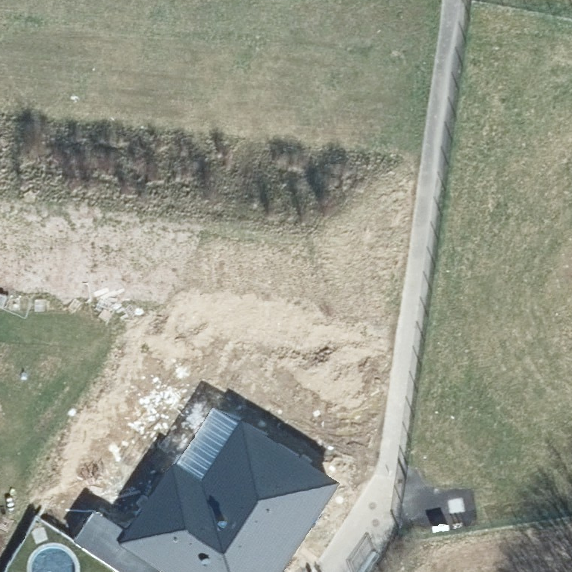
\includegraphics[width=\LabelConsiderationImageWidth]{images/consideration_labels/44883}
    \hspace{1mm}
    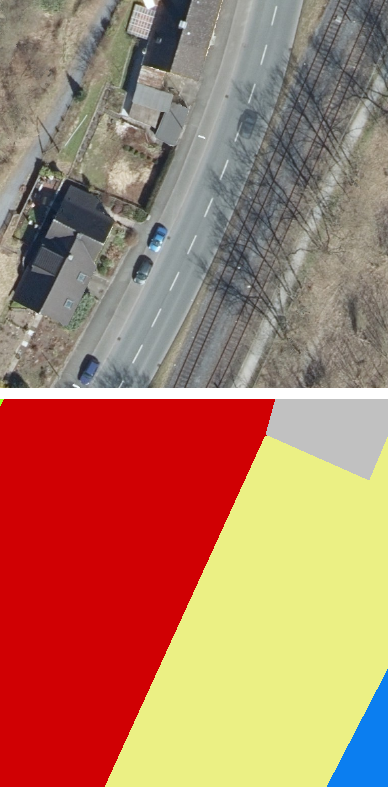
\includegraphics[width=\LabelConsiderationImageWidth]{images/consideration_labels/150815}
    \hspace{1mm}
    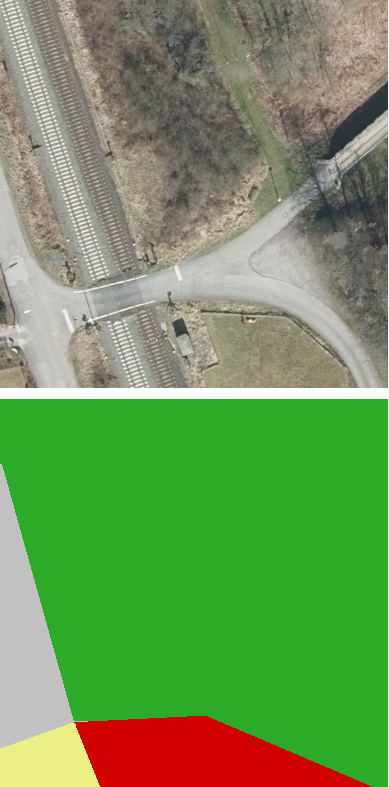
\includegraphics[width=\LabelConsiderationImageWidth]{images/consideration_labels/69493}
    \hspace{1mm}
    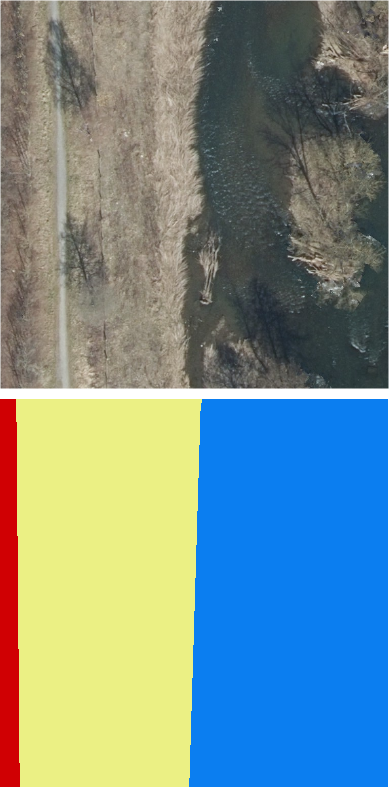
\includegraphics[width=\LabelConsiderationImageWidth]{images/consideration_labels/71270}

    \vspace{3mm}

    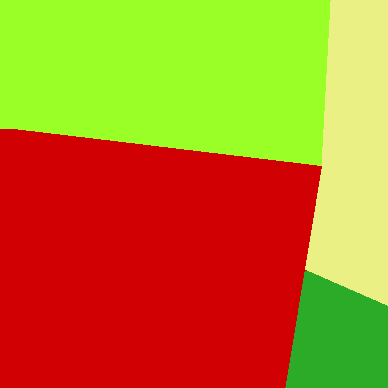
\includegraphics[width=\LabelConsiderationImageWidth]{images/consideration_labels/44883-label}
    \hspace{1mm}
    
\includegraphics[width=\LabelConsiderationImageWidth]{images/consideration_labels/150815-label}
    \hspace{1mm}
    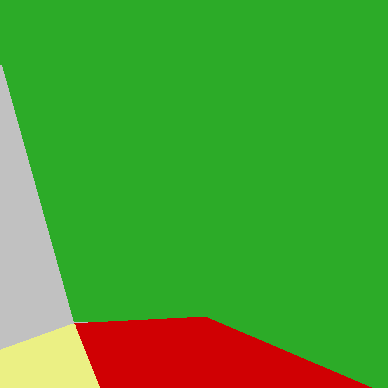
\includegraphics[width=\LabelConsiderationImageWidth]{images/consideration_labels/69493-label}
    \hspace{1mm}
    
\includegraphics[width=\LabelConsiderationImageWidth]{images/consideration_labels/71270-label}

    \caption{Poorly outlined edges on adjacent segments}
    \label{fig:label_considerations}
\end{figure}

To get really good predictions, training should ideally be performed with pixel-perfect labels. For this thesis, pixel-perfect predictions are not aspired. To identify emergency landing fields, we are looking for large contiguous areas, so minor inaccuracies at the edges might not be an issue. However, it is very likely that the inaccurate training data affects the quality of the predictions. This is something to keep in mind when evaluating the performance of the trained models.

\newpage
